\section{Screening}
\subsection{General Definitions and Setup of Problem}
For definitions and general discussion, see Ashcroft and Mermin p.337-339.

\begin{figure}[htbp]
    \centering
    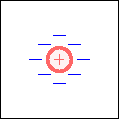
\includegraphics[]{Images/fig-screeningcartoon.pdf}
    \caption{Cartoon of electron screening; when a positive test charge is placed in a cloud of negative charge, the negative charges are attracted to the positive charge. This has the net effect of screening out the positive charge, as it gets neutralized to some capacity.}
    \label{fig-screeningcartoon}
\end{figure}
If we place a (positive) test charge in an cloud of negative charge, then it attracts negative charges around it, which results in a net screening of the positive charge. 

We have the potentials $\phi^{ext}, \phi$ and the charge densities $\rho^{ext}, \rho, \rho^{ind} = \rho - \rho^{ext}$. 

\begin{equation}\label{eq-potentialsdielectric}
    \begin{split}
        \phi(\v{q}) &= \frac{1}{\e(\v{q})}\phi^{ext}(\v{q})
        \\ \rho^{ind}(\v{q}) &= \chi(\v{q})\phi(\v{q})
        \\ \e(\v{q}) &= 1 - \frac{4\pi}{q^2}\chi(\v{q})
    \end{split}
\end{equation}
where $\e(\v{q})$ is the dielectric function and $\chi(\v{q})$ is the dielectric susceptibility. 

Today, we will go through two different calculations of the susceptibility.

\subsection{Thomas-Fermi Theory}
We have the second-quantized Hamiltonian:
\begin{equation}
    \begin{split}
        &\hat{H} = \int d^3x\hat{\psi}^\dag(\v{x})T(\v{x})\hat{\psi}(\v{x})
        \\ &T(\v{x}) = \frac{\hbar^2\nabla^2}{2m} - e\phi(\v{x})
    \end{split}
\end{equation}
we neglect $e-e$ interactions (including them makes this much more difficult). Of course electrons will see the total screened potential rather than the bare test charge potential, which this formula accounts for ($\phi$ vs. $\phi^{ext}$). 

For $\phi(\v{x}) = \phi_0$ a constant, we can solve the problem exactly. The Hamiltonian becomes:
\begin{equation}
    H = \sum_{\v{k}}\left(\frac{\hbar^2\v{k}^2}{2m} - e\phi_0\right)c_\v{k}^\dag c_\v{k} = \sum_{\v{k}}\e_\v{k}c_\v{k}^\dag c_\v{k}.
\end{equation}
Thomas-Fermi theory assumes that $\phi(\v{x})$ varies slowly on the scale $k_F^{-1}$; therefore in a semiclassical approximation, it is appropriate to write:
\begin{equation}
    \e_\v{k} \to \frac{\hbar^2\v{k}^2}{2m} - e\phi_0
\end{equation}
We will calculate the local electron density at $\v{r}$. It will be given by:
\begin{equation}\label{eq-screeningchargedensity}
    \begin{split}
        \rho(\v{r}) &= -e\avg{\hat{\psi}^\dag(\v{r})\hat{\psi}(\v{r})}
        \\ &= -2e\sum_{\v{k}\v{k}'}\avg{\hat{\psi}_{\v{k}}^\dag(\v{r})\hat{\psi}_{\v{k}'}(\v{r})c^\dag_{\v{k}}c_{\v{k}'}}
        \\ &= -2e\sum_{\v{k}\v{k}'}\hat{\psi}_{\v{k}}^\dag(\v{r})\hat{\psi}_{\v{k}'}(\v{r})\avg{c^\dag_{\v{k}}c_{\v{k}'}}
        \\ &= -2e\sum_{\v{k}\v{k}'}\hat{\psi}_{\v{k}}^\dag(\v{r})\hat{\psi}_{\v{k}'}(\v{r})\delta_{\v{k}\v{k}'}f(\e_{\v{k}}(\v{r}))
        \\ &= -2e\sum_{\v{k}}\abs{\psi_{\v{k}}(\v{r})}^2f(\e_{\v{k}}(\v{r}))
    \end{split}
\end{equation}
where the factor of $2$ comes from counting the two possible spin states, $f(\e_{\v{k}}(\v{r}))$ is the Fermi-Dirac distribution (which comes from the fact that at any temperature, the expectation value of the number of fermions of any state at a given energy is given from stat mech to be the FD distribution; previously we denoted this as $n_{\v{k}}$. For bosons next week it will be the BE-distribution), and in the last equality we use the Kronecker delta to perform the last of the summations. For the plane wave basis, we have $\psi_{\v{k}}(\v{r}) = \frac{1}{\sqrt{V}}e^{-i\v{k} \cdot \v{r}}$, so:
\begin{equation}
    \begin{split}
        \rho(\v{r}) &= -\frac{2e}{V}\sum_{\v{k}}\frac{1}{e^{\beta(\e_{\v{k}}(\v{r}) - \mu) + 1} + 1}
        \\ &= -en_0(\mu + e\phi(\v{r}))
    \end{split}
\end{equation}
where $\beta = \frac{1}{k_B T}$ as usual, and we define:
\begin{equation}
    n_0(\mu) = \int \frac{d^3k}{4\pi^3}\frac{1}{e^{\beta(\frac{\hbar^2\v{k}^2}{2m} - \mu) + 1} + 1}.
\end{equation}
We can now write the induced charge density as:
\begin{equation}\label{eq-rhoind}
    \rho^{ind}(\v{r}) = -e\left[n_0(\mu + e\phi(\v{r})) - n_0(\mu)\right] \approx -e^2\phi(\v{r})\dpd{n_0}{\mu}.
\end{equation}
which is just the difference between the total charge density and the average charge density in the sample (with no test charge), and we make the approximation that not only is $\phi$ slowly varying, but in itself small, allowing us to take the first-order Taylor approximation to $\rho^{ind}$ and neglect the higher-order terms.

Now, comparing Eqs. \eqref{eq-potentialsdielectric} and \eqref{eq-rhoind}, we can read off the dielectric susceptibility (and the function):
\begin{equation}\label{eq-TFresult}
    \boxed{\begin{split}
        \chi(\v{q}) &= -e^2\dpd{n_0}{\mu}
    \\ \e(\v{q}) &= 1 + \frac{4\pi e^2}{q^2}\dpd{n_0}{\mu}
    \end{split}}
\end{equation}
this is the main result of Thomas-Fermi theory of electron screening.

\subsection{Implications of Thomas-Fermi Theory}
Some housekeeping; Eq. \eqref{eq-TFresult} is often stated in the form:
\begin{equation}
    \e(\v{q}) = 1 + \frac{k_{TF}^2}{q^2}, \quad k_{TF} = 4\pi e^2\dpd{n_0}{\mu}.
\end{equation}
$k_{TF}$ is called the Thomas-Fermi momentum, and gives us a length scale for which the test charge is screened out. We illustrate the significance of $k_{TF}$ by considering the screened potential of a point charge:
\begin{equation}
    \phi^{ext}(\v{r}) = \frac{Q}{r} \to \phi^{ext}(\v{q}) = \frac{4\pi Q}{q^2}
\end{equation}
\begin{equation}
    \phi(\v{r}) = \frac{1}{\e(\v{q})}\phi^{ext}(\v{q}) = \frac{4\pi Q}{q^2 + k_{TF}^2}
\end{equation}
In real space, this becomes:
\begin{equation}
    \phi(\v{r}) = \int \frac{d^3}{(2\pi)^3}e^{i\v{q} \cdot \v{r}}\frac{4\pi Q}{q^2 + k_{TF}^2} = \frac{Q}{r}e^{-k_{TF}r}
\end{equation}
where the integral can be done by going into spherical coordinates. This is a very important result which tells us how screening acts in our simple Thomas-Fermi theory (though it is true more generally). This is known as the screened Coulomb, or Yukawa potential (often used in nuclear physics, though its origin is not electrostatic but nuclear). The presence of electrons exponentially supresses the test charge with distance, in particular the potential rapidly vanishes at distances $r > k_{TF}^{-1} = \lambda_{TF}$ which we call the screening length.

We may recall that we found a singularity in the derive in the effective dispersion when we covered Hartree-Fock theory. This was due to the long range interactions; but if one accounts for the screening/exponential suppression, then this singularity goes away.

As a last step, let us estimate the size of $\lambda_{TF}$ in a metal. We have that:
\begin{equation}
    \dpd{n_0}{\mu} = -\int \frac{d^3k}{4\pi^3}\dpd{}{\mu}\left[\frac{1}{e^{\beta(\e_\v{k} - \mu)} + 1}\right] \longrightarrow^{T \to 0} \int \frac{d^3k}{4\pi^3}\delta(\e_{\v{k}} - \mu) = g(\mu) = \frac{mk_F}{\hbar^2 \pi^2}
\end{equation}
where the last quantity is just the density of states at the Fermi level in 3-D. Sticking this into the result for $k_{TF}$, we get:
\begin{equation}
    \frac{k_{TF}^2}{k_F^2} = \frac{4}{\pi}\frac{me^2}{\hbar^2k_F} = \frac{4}{\pi} \frac{1}{a_0k_F} = \left(\frac{16}{3\pi^2}\right)^{3/2}r_s \implies k_{TF} = 0.815k_F\sqrt{r_s} \implies \lambda_{TF} \approx k_{F}^{-1} = \frac{\sqrt{r_s}}{2.95}A^{\circ}
\end{equation}
This tells us that in a metal (where $r_s = 2-6$), the Coulomb interaction is screened at very short distances, comparable to the ionic spacings.

A comment: We have made the semiclassical assumption that $\phi$ varies slowly; but it does not vary slowly on the given length scale. It's not valid in real materials, but it is still a useful result. 

\subsection{Lindhard Theory}
In the Lindhard theory, we assume that $\phi(\v{r})$ is small and can be treated as a perturbation:
\begin{equation}
    H = \frac{\hbar^2 \nabla^2}{2m} - e\phi(\v{r})
\end{equation}
where the first term is $H_0$ and the second is $H_1$. This approximation is almost always valid. We calculate the charge density using Eq. \eqref{eq-screeningchargedensity}. We will need to find the correction to $\psi_{\v{k}}(\v{r})$ due to perturbation. This correction looks like:
\begin{equation}
    \psi_{\v{k}}(\v{r}) = \psi_{\v{k}}^0(\v{r}) + \sum_{\v{k}'}\frac{\bra{\psi^0_{\v{k}'}}-e\phi(\v{r})\ket{\psi^0_{\v{k}'}}}{\e_{\v{k}} - \e_{\v{k}'}}\psi_{\v{k}'}^0(\v{r}) + \ldots
\end{equation}
Now, since:
\begin{align*}
    \psi_{\v{k}}^0(\v{r}) = \frac{1}{\sqrt{V}}e^{i\v{k} \cdot \v{r}}, \quad \e^0_{\v{k}} = \frac{\hbar^2\v{k}^2}{2m}
\end{align*}
we have:
\begin{equation}
    \bra{\psi_\v{k}'^0}-e\phi(\v{r})\ket{\psi_{\v{k}}^0} = -\frac{e}{V}\int d^3r e^{-i\v{k}' \cdot \v{r}} \phi(\v{r})e^{i\v{k} \cdot \v{r}} = -\frac{e}{V}\phi(\v{k} - \v{k}')
\end{equation}
where in the last equality we recognize the operation being carried out as a Fourier transform. We now have:
\begin{equation}
    \psi_\v{k}(\v{r}) = \psi_{\v{k}}^0(\v{r}) - \frac{e}{V}\sum_{\v{k}'}\frac{\phi(\v{k} - \v{k'})}{\e^0_{\v{k}} - \e^0_{\v{k}'}}\psi^0_{\v{k}'}(\v{r})
\end{equation}
We then substitute $\psi_\v{k}(r)$ into Eq. \eqref{eq-screeningchargedensity} and retain terms up to first order in $\phi(\v{k} - \v{k}')$. This yields:

\begin{equation}
    \rho(\v{r}) = -e\left[\sum_{\v{k}}f_k\abs{\psi_\v{k}^0}^2 - \frac{e}{V}\sum_\v{k}\left(f_\v{k}\psi_\v{k}^{0*}\sum_{\v{k}'} \frac{\psi^0_{\v{k}'}}{\e^0_\v{k} - \e^0_{\v{k}'}}\phi(\v{k} - \v{k}') + c.c.\right)\right]
\end{equation}

Where the first term is $\rho_0(\v{r})$ and the second term is $\rho^{ind}(\v{r})$. $f_\v{k}$ is the Fermi-dirac distribution for energy $\e_{\v{k}}$. We can evaluate this integral using the substitution:
\begin{align*}
    (\v{k}, \v{k}') \to (\v{k} + \frac{1}{2}\v{q}, \v{k} - \frac{1}{2}\v{q})
\end{align*}
We then obtan:
\begin{equation}
    \rho^{ind}(\v{r}) = -\frac{e^2}{V}\sum_{\v{q}}e^{i\v{q} \cdot \v{r}}\left(\sum_{\v{k}} \frac{f_{\v{k} + \frac{1}{2}\v{q}} - f_{\v{k} - \frac{1}{2}\v{q}}}{\e^0_{\v{k} + \frac{1}{2}\v{q}} - \e^0_{\v{k} - \frac{1}{2}\v{q}}}\right) \phi(\v{q})
\end{equation}
we can therefore conclude that $\rho^{ind}(\v{q}) = \chi(\v{q})\phi(\v{q})$, where:
\begin{equation}
    \boxed{\chi(\v{q}) = -\frac{e^2}{V}\sum_{\v{k}} \frac{f_{\v{k} + \frac{1}{2}\v{q}} - f_{\v{k} - \frac{1}{2}\v{q}}}{\e^0_{\v{k} + \frac{1}{2}\v{q}} - \e^0_{\v{k} - \frac{1}{2}\v{q}}}}
\end{equation}
This is our final result, the Lindhard susceptibility function. WE note that $\chi(\v{q})$ looks different from the Thomas-Fermi case, and there is an explicit dependence of $\chi(\v{q})$ on $\v{q}$. 

\subsection{Limits of the Lindhard Results}
We look at two limits. At low $T$ and small $q$, the numerator is small unless $\abs{\v{k}} \approx k_F$ (we subtract two near-step functions in the numerator, and the difference is only nonzero for $\abs{\v{k}} \approx k_F$). Therefore we can expand:
\begin{equation}
    f_{\v{k} \pm \frac{1}{2}\v{q}} \approx f_\v{k} \pm \frac{\hbar^2}{2}\frac{\v{k} \cdot \v{q}}{m}\dpd{f_\v{k}}{\mu} + O(q^2)
\end{equation}
so we get:
\begin{equation}
    \chi(\v{q}) \approx -\frac{e^2}{V}\sum_{\v{k}}\dpd{f_\v{k}}{\mu}
\end{equation}
we recover the TF result! This makes sense, as the small $q$ limit is the large-wavelength limit, i.e. $\phi$ varies slowly.

At $T = 0$, the $\v{k}$ integral can be evaluated exactly:
\begin{equation}
    \chi(\v{q}) = -e^2\left(\frac{mk_F}{\pi^2\hbar^2}\right)\left[\frac{1}{2} + \frac{1-x^2}{4x^2}\ln\left|\frac{1+x}{1-x}\right|\right]
\end{equation}
where $x = q/2k_F$. This is the same function that appeared in our discussion of Hartree-Fock, and it is non-analytic at $x = 1$. Because the dielectric function $\e(\v{q}) = 1 - \frac{4\pi}{q^2}\chi(\v{q})$ is non-analytic at $q \to 2k_F$, it is possible to show that the screened potential of a point charge contains a term:
\begin{equation}
    \phi(\v{r}) \approx \frac{1}{r^3}\cos(2k_F r)
\end{equation}
for $r \gg k_F^{-1}$. This is known as the ``Friedel'', or ``RKKY'' oscillation (so to recap, we have an exponetially decaying term, and we also have a power-law decaying oscillatory term). It is observable experimentally, using STM.

Why is this? Electrons come in to screen the test charge, but ``overscreen'', creating a region of high negative charge density. So then the electrons go away from this region to compensate, and this leads to this oscillatory effect.

Next class, we study bosonic excitations in solds.